\section{The Dataset}

\begin{frame}{Problem Setting}
	\begin{block}{}
		We define the multimodal input space as the Cartesian product of $P$ modality-specific input spaces:
		\[
		\mathcal{X} = \prod_{p=1}^{P} \mathcal{X}^{(p)},
		\]
		where each modality $\mathcal{X}^{(p)}$ may represent data from distinct sources.
	\end{block}
	
\end{frame}



\begin{frame}{Toadstool 2 Dataset}
\begin{block}{}
The dataset consists of video, sensor, and demographic data collected from 10 participants playing a Super Mario Bros.
\end{block}


		\begin{columns}[T] % Top alignment
		\begin{column}{0.5\textwidth}
			\begin{center}
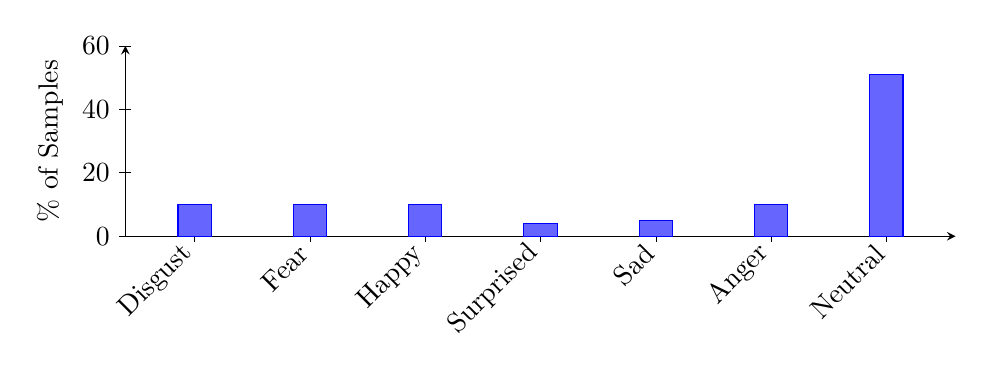
\begin{tikzpicture}
	\begin{axis}[
		width=\textwidth,
		height=4cm,
		ybar,
		bar width=12pt,
		axis lines=left,
		ylabel={\% of Samples},
		symbolic x coords={Disgust,Fear,Happy,Surprised,Sad,Anger,Neutral},
		xtick=data,
		xticklabel style={rotate=45, anchor=east},
		ymin=0, ymax=60,
		tick style={black},
		enlarge x limits=0.1  % adds horizontal margin on both sides
		]
		\addplot+[fill=blue!60] coordinates {
			(Disgust,10) (Fear,10) (Happy,10)
			(Surprised,4) (Sad,5) (Anger,10) (Neutral,51)
		};
	\end{axis}
\end{tikzpicture}

			\end{center}
			
		\end{column}
		\begin{column}{0.5\textwidth}

		\begin{block}{}
	We focus on sensor data. We get a total of 20970 samples corresponding to a label taking in a 4s time window.
\end{block}
		\centering
		\small
		\begin{tabular}{lcc}
		\toprule
		\textbf{Signal} & \textbf{Rate (Hz)} & \textbf{Channels} \\
		\midrule
		BVP  & 64 & 1      \\
		ACC  & 32 & 3 		\\
		EDA  & 4  & 1      \\
		HR   & 1  & 1      \\
		\bottomrule
		\end{tabular}
		



		\end{column}
	\end{columns}
\end{frame}


\begin{frame}{Toadstool 2 Dataset}
	
	\begin{block}{Dataset Overview}
		Sensor and demographic data recorded from 10 participants during Super Mario Bros gameplay. 
	\end{block}
	
	\begin{columns}[T]
		
		\begin{column}{0.48\textwidth}
			\begin{block}{Class Distribution}
				Most samples (51\%) are neutral. Other classes evenly distributed (~10\% each), except \textit{Surprised} (4\%) and \textit{Sad} (5\%).
			\end{block}
			\vspace{1ex}
			\centering
			\small
			\begin{tabular}{ll}
				\toprule
				\textbf{Emotion} & \textbf{Samples (\%)} \\
				\midrule
				Disgust & 10\% \\
				Fear & 10\% \\
				Happy & 10\% \\
				Surprised & 4\% \\
				Sad & 5\% \\
				Anger & 10\% \\
				Neutral & 51\% \\
				\bottomrule
			\end{tabular}
		\end{column}
		
		\begin{column}{0.52\textwidth}
			\begin{block}{Sensor Data}
				\textbf{Total samples:} 20,970 (4\,s windows per sample).
			\end{block}
			\vspace{1ex}
			\centering
			\small
			\begin{tabular}{lcc}
				\toprule
				\textbf{Sensor} & \textbf{Hz} & \textbf{Channels} \\
				\midrule
				BVP & 64 & 1 \\
				ACC & 32 & 3 \\
				EDA & 4 & 1 \\
				HR & 1 & 1 \\
				\bottomrule
			\end{tabular}
		\end{column}
		
	\end{columns}
	
\end{frame}



